\documentclass[10pt, landscape]{article}
\usepackage[scaled=0.92]{helvet}
\usepackage{calc}
\usepackage{multicol}
\usepackage{ifthen}
\usepackage[a4paper,margin=5mm,landscape]{geometry}
\usepackage{amsmath,amsthm,amsfonts,amssymb}
\usepackage{color,graphicx,overpic}
\usepackage{hyperref}
\usepackage{newtxtext} 
\usepackage{enumitem}
\usepackage{amssymb}
\usepackage[table]{xcolor}
\usepackage{vwcol}
\usepackage{tikz}
\usetikzlibrary{arrows.meta}
\usetikzlibrary{calc}
\usepackage{mathtools}
\usepackage{nicematrix}
\usepackage[T1]{fontenc} %%% <--- NOTE THIS
% for relations
\usepackage{cancel}
\usepackage{ mathrsfs }
\usepackage{listings}
\usepackage{background}
\setlist{nosep}

\usepackage{etoolbox}
\makeatletter
\preto{\@verbatim}{\topsep=0pt \partopsep=0pt }
\makeatother

\backgroundsetup{
scale=1,
color=black,
opacity=0.3,
angle=0,
contents={}
% {
\includegraphics[width=\paperwidth,height=\paperheight]{tux.png}}
}

\pdfinfo{
  /Title (CS2106.pdf)
  /Creator (TeX)
  /Producer (pdfTeX 1.40.0)
  /Author (Seamus)
  /Subject (Example)
  /Keywords (pdflatex, latex,pdftex,tex)}

\lstset{language=Java,keywordstyle={\bfseries \color{black}}}

% Turn off header and footer
\pagestyle{empty}

\newenvironment{tightcenter}{%
  \setlength\topsep{0pt}
  \setlength\parskip{0pt}
  \begin{center}
}{%
  \end{center}
}

% redefine section commands to use less space
\makeatletter
\renewcommand{\section}{\@startsection{section}{1}{0mm}%
                                {-1ex plus -.5ex minus -.2ex}%
                                {0.5ex plus .2ex}%x
                                {\normalfont\large\bfseries}}
\renewcommand{\section}{\@startsection{section}{2}{0mm}%
                                {-1explus -.5ex minus -.2ex}%
                                {0.5ex plus .2ex}%
                                {\normalfont\normalsize\bfseries}}
\renewcommand{\subsection}{\@startsection{subsection}{3}{0mm}%
                                {-1ex plus -.5ex minus -.2ex}%
                                {1ex plus .2ex}%
                                {\normalfont\small\bfseries}}%
\renewcommand{\familydefault}{\sfdefault}
\renewcommand\rmdefault{\sfdefault}
% makes nested numbering (e.g. 1.1.1, 1.1.2, etc)
\renewcommand{\labelenumii}{\theenumii}
\renewcommand{\theenumii}{\theenumi.\arabic{enumii}.}
\renewcommand\labelitemii{•}
%  for logical not operator
\renewcommand{\lnot}{\mathord{\sim}}
\renewcommand{\bf}[1]{\textbf{#1}}
\newcommand{\abs}[1]{\vert #1 \vert}
\newcommand{\Mod}[1]{\ \mathrm{mod}\ #1}

\makeatother
\definecolor{myblue}{cmyk}{1,.72,0,.38}
\everymath\expandafter{\the\everymath \color{myblue}}
% Define BibTeX command
\def\BibTeX{{\rm B\kern-.05em{\sc i\kern-.025em b}\kern-.08em
    T\kern-.1667em\lower.7ex\hbox{E}\kern-.125emX}}
\let\iff\leftrightarrow
\let\Iff\Leftrightarrow
\let\then\rightarrow
\let\Then\Rightarrow

% Don't print section numbers
\setcounter{secnumdepth}{0}

\setlength{\parindent}{0pt}
\setlength{\parskip}{0pt plus 0.5ex}
%% this changes all items (enumerate and itemize)
\setlength{\leftmargini}{0.5cm}
\setlength{\leftmarginii}{0.5cm}
\setlist[itemize,1]{leftmargin=2mm,labelindent=1mm,labelsep=1mm}
\setlist[itemize,2]{leftmargin=4mm,labelindent=1mm,labelsep=1mm}

%My Environments
\newtheorem{example}[section]{Example}
% -----------------------------------------------------------------------

\begin{document}
\raggedright
\footnotesize
\begin{multicols*}{3}

% multicol parameters
% These lengths are set only within the two main columns
\setlength{\columnseprule}{0.25pt}
\setlength{\premulticols}{1pt}
\setlength{\postmulticols}{1pt}
\setlength{\multicolsep}{1pt}
\setlength{\columnsep}{2pt}

\begin{center}
    \fbox{%
        \parbox{0.8\linewidth}{\centering \textcolor{black}{
            {\Large\textbf{CS2106}}
            \\ \normalsize{AY25/26 Sem 1}}
            \\ {\footnotesize \textcolor{myblue}{by ngmh}} 
        }%
    }
\end{center}

% \section{Introduction}
% \begin{itemize}
%     \item Operating System: Program that acts as an intermediary between a computer user and computer hardware
%     \item First Computers: No OS, directly interact and change hardware, minimal overhead, but inefficient and not portable
%     \item Mainframes: Accept programs in physical form, only support batch processing, very costly
%     \item Batch OS: Execute user program / job one at a time, still interacts with hardware directly, with additional information for OS such as required resources and job specification
%     \item Batch processing is inefficient: CPU idle when performing I/O
%     \item Can use multiprogramming to load multiple jobs at once to pipeline, overlapping computation and I/O
%     \item Time-Sharing OS: Allow multiple users to interact with machine using terminals / teletypes, user job scheduling gives illusion of concurrency, supports memory management
%     \item Personal OS: Machine dedicated to user, not timeshared
% \end{itemize}

% \subsection{Motivation}
% \begin{itemize}
%     \item Abstraction: Hide low level details and present common high level functionality to user
%     \item Large variation in hardware configurations and low-level details which user might not be interested in
%     \item Resource Allocator: OS manages all resources and arbitrates conflicting requests for efficient and fair use
%     \item Control Program: OS controls execution to prevent errors and improper use, providing security, isolation and protection
%     \item Improves Program Portability and Efficiency
% \end{itemize}

\subsection{Operating Systems}
\begin{itemize}
    \item OS is software that runs in kernel mode with direct access to hardware resources, other software runs in user mode
    \item User programs call OS using system call interface
    \item Kernel is a program with special features to deal with hardware and provide the syscall interface, with special code for interrupt handlers and device drivers
    \item Kernel code cannot use syscalls, normal libraries, or I/O
    % \item Programming Language for OS: Historically in assembly, but now in higher level languages like C/C++, hardware architecture dependent
    % \item Code Organisation: Machine independent / dependent HLL / assembly code
    \item Virtualisation: each program executes as if it has all resources to itself
\end{itemize}

\subsection{OS Structures}
\begin{itemize}
    \item Monolithic: Kernel is one big special program, various services and components are integral part
    \item Good performance but complicated internal structure with highly coupled components
    \item Microkernel: Small and clean, only provides basic and essential facilities such as IPC, address space and thread management
    \item Higher level services are built on top, and run as server process outside of OS, using IPC to communicate
    \item More robust and extendible, with better isolation and protection, but lower performance
    \item Others include layered systems or client-server model
    % \item Layered Systems: Generalisation of Monolithic System, organising components into hierarchy of layers with lowest being hardware and highest being user interface
    % \item Client-Server Model: Variation of microkernel, with two classes of processes; Client process request service from server process, which is built on top of microkernel, can even be on different machines
\end{itemize}

\subsection{Virtual Machines}
\begin{itemize}
    \item Allows us to run multiples OSes on the same hardware at the same time, as well as debug / monitor them
    \item Virtual Machine: Software emulation / virtualisation of hardware, created and managed by hypervisor / Virtual Machine Monitor
    \item Type 1 Hypervisor: Provides individual virtual machines to guest OSes, bare metal hypervisor directly on hardware
    \item Type 2 Hypervisor: Runs in host OS, guest OS runs inside virtual machine
\end{itemize}

\section{Process Abstraction}
\subsection{Memory Context: Function Call}
\begin{itemize}
    % \item Important Steps
    % \begin{itemize}
    %     \item Setup parameters
    %     \item Transfer control to callee
    %     \item Setup local variables
    %     \item Store result if applicable
    %     \item Return to caller
    % \end{itemize}
    % \item Control Flow issues: Need to jump to function body, and resume when function call is done; minimally need PC of caller
    % \item Data Storage issues: Need to pass parameters to the function, and capture return result, function might also have local variables
    % \item Need a new region of memory that is dynamically used by function invocations
    \item Stack Memory: New memory region to store information for a function invocation, described by a stack frame
    \item Stack Frame contains ra / PC, arguments / parameters, storage for local variables, other info
    \item Stack Pointer: Points to first unused location, usually in a specialised register
    \item Function Call Convention (Different ways to setup stack frame)
    \begin{itemize}
        \item Prepare to make call: Caller passes parameters with registers or stack, then saves return PC on stack
        \item Transfer control to callee: Callee saves old stack pointer, allocates space for local variables, and adjusts stack pointer to new stack top
        \item On returning from function call: Callee places return result in register, and restores saved stack pointer
        \item Transfer control back to caller using saved PC: Caller utilises return result, and continues execution
    \end{itemize}
    \item Other information: Frame pointer, saved registers
    \item Frame Pointer: Facilitates access of various stack frame items, might be dedicated register, points to fixed location in a stack frame so that other items can be accessed as a displacement from it, each stack frame has one
    \item Saved registers: Use memory to hold GPR values when exhausted, so it can be used and restored, known as register spilling
    \item Function can spill registers it intends to use before function starts, to be restored at end of function
    \item Updated Steps
    \begin{itemize}
        \item Prepare to make call: Caller passes parameters with registers or stack, then saves return PC on stack
        \item Transfer control to callee: Callee saves registers used by callee, old stack pointer, old frame pointer, allocates space for local variables on stack, and adjusts stack pointer to new stack top, adjusts frame pointer
        \item On returning from function call: Callee restores saved registers, FP, SP, places return result in register
        \item Transfer control back to caller using saved PC: Caller utilises return result, and continues execution
    \end{itemize}
    \item Stack Frame Illustration:
    \begin{itemize}
        \item Free Memory; Local Variables (Stack pointer points above here)
        \item Parameters; Saved Registers
        \item Saved SP (Top of previous stack frame), (Frame pointer points above here)
        \item Saved FP (Base address of previous stack frame)
        \item Return PC
    \end{itemize}
    \item Text memory: For instructions
    \item Data memory: For global / static variables
\end{itemize}

% \subsection{Dynamically Allocated Memory}
% \begin{itemize}
    % \item Memory space acquired during execution time
    % \item Blocks allocated at runtime cannot be placed in data region
    % \item Blocks with no definite deallocation timing cannot be placed in stack region
    % \item Create separate heap memory for dynamic allocation
    % \item Heap memory is harder to manage due to variable size and allocation/deallocation, and adverse scenarios can be constructed
%     \item Text memory: For instructions
%     \item Data memory: For global / static variables
% \end{itemize}

\subsection{Process Management}
\begin{itemize}
    % \item To switch between programs, OS requires information regarding execution of current program to be stored, and replaced with new information for next program to run
    % \item Need abstraction to describe a running program, known as process
    % \item Process Abstraction: Process / Task / Job is a dynamic abstraction for executing program, includes memory, hardware, OS context
    \item Process ID: Used to distinguish processes from each other, unique
    \item Process State: Processes can be either running, or not running, but can also be in a ready state
    \item Process Model: Set of states and transitions
    \item 5-Stage Model: New, Ready, Running, Blocked, Terminated
    % \begin{itemize}
    %     \item New process created, undergoes intialisation
    %     \item Ready: Process is waiting to be run
    %     \item Running: Process is being executed on CPU
    %     \item Blocked: Process waiting / sleeping for event, cannot execute until event is available e.g. syscall, I/O
    %     \item Terminated: Process finished execution, might need OS cleanup
    % \end{itemize}
    \item Queuing Model: OS has ready and blocked queue with processes inside, awaiting execution
% \end{itemize}
% \begin{center}
%     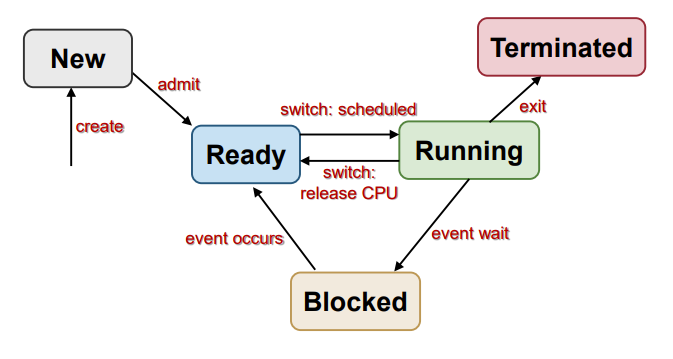
\includegraphics[width=\linewidth]{5states.png}
% \end{center}

% \subsection{Process Table and Control Block}
% \begin{itemize}
    \item Process Control Block (PCB) or Process Table Entry: Entire execution context for a process
    \item Kernel maintains PCB for all processes in a table
    \item Issues: Scalability and Efficiency
\end{itemize}

\subsection{System Calls}
\begin{itemize}
    % \item API to OS, not same as normal function call, must change from user mode to kernel mode
    % \item API is dependent on OS
    % \item In C/C++, system calls can be invoked almost directly with library version acting as function wrapper
    % \item Some library functions are more user friendly and serve as function adapters, not one to one
    \item General System Call Mechanism
    \begin{itemize}
        \item User program invokes library call using normal function call mechanism
        \item Library call (usually in assembly) places system call number in designated location such as register
        \item Library call executes special instruction (TRAP) to switch from user to kernel mode, saves CPU state
        \item Appropriate system call handler is determined, using system call number as index, handled by dispatcher
        \item System call handler is executed
        \item System call handler ends, restores CPU state, returns to library call, switch back to user mode
        \item Library call returns to user program via normal function return mechanism
    \end{itemize}
\end{itemize}

\subsection{Exception and Interrupt}
\begin{itemize}
    \item Exceptions can be caused by executing machine level instructions, e.g. Arithmetic / Memory Access errors
    \item Exceptions are synchronous, occurring due to execution
    \item Exception handler is executed, similar to a forced function call
    \item Interrupts are external events that can interrupt the execution of a program, usually hardware related
    \item Interrupts are asynchronous, independent of program execution
    \item Program execution is suspended, and an interrupt handler must be executed
    \item Control transfer to handler routine automatically, before being returned to
\end{itemize}

\subsection{Process Abstraction in Unix}
\begin{itemize}
    \item Processes are identified by integer Process IDs
    \item Information: Process State (Running, Sleeping, Stopped, Zombie), Parent PID, Cumulative CPU time
    \item Process creation: Using fork(), duplicates executable image, copy on write
    % \item Creates a new child process which is duplicate of current executable image, data is a copy of parent (copy on write)
    \item Child only differs in PID, PPID, and fork() return value (PID of new process for parent, 0 for child)
    \item Both continue execution after fork()
    \item For a different program, can use exec() variations instead
    % \item \verb|execl(path, arg0, arg1, NULL)|: Replace current executing process image with a new one, code replacement, PID and other information intact, pass in path and arguments
    \item Master process: init, created in kernel at boot up, has PID 1, forms process tree
    \item Use exit() to end execution of process, 0 is normal exit
    \item On finish, most system resources used are released such as file descriptors, while basic process resources are not like PID and status as well as process accounting info since process table entry might still be needed
    \item Parent Child Synchronisation: Parent process waits for \textbf{immediate child process} to terminate using \verb|wait(int *status)|
    \item Wait is blocking until at least one child terminates, and cleans up remainder of child system resources, has other variations as well
    \item On process exit, zombie is created since not all process info is deleted, wait() cleans it up
    \item Orphan: Parent terminates before child process: init becomes psuedo parent, then child termination sends signal to init which cleans it up with wait()
    \item Zombie: Child process terminates before parent, who did not wait(): Child becomes a zombie, and can fill up process table
\end{itemize}

\subsubsection{Implementation of fork()}
\begin{itemize}
    \item Makes an almost exact copy of parent process
    \begin{itemize}
        \item Create address space of child process
        \item Allocate new PID
        \item Create kernel process data structures like entry in process table
        \item Copy kernel environment of parent process such as priority
        \item Initialise child process context like PID, PPID, CPU time
        \item Copy memory regions from parent such as Program, Data, Stack, but this is expensive
        \item Acquire shared resources like open files, current working directory
        \item Initialise hardware context for child processes by copying registers from parent process or others
        \item Add child process to scheduler queue to wait to be run
    \end{itemize}
    % \item Memory Copy is expensive, as potentially the whole memory space needs to be copied
    % \item However, child process will not access the whole memory range immediately, and shared version can be used if read only
    \item Copy on Write: Only duplicate a memory location when written to
    \item Memory is stored in memory pages and managed on a page level instead
\end{itemize}

\section{Process Scheduling}

\subsection{Concurrent Execution}
\begin{itemize}
    \item Concurrent Processes: Multiple processes progress in execution at the same time, could be virtual or physical
    \item Timeslicing: Using 1 CPU, interleave instructions from both processes
    \item Multitasking needs to change context between processes, which incurs overhead
    \item Multiprocessor: Timeslicing on multiple CPUs at the same time
    \item Scheduling: How to organise processes to run
    \item Scheduler: Part of OS which makes scheduling decision
    \item Scheduling Algorithm: Algorithm used by scheduler
    \item Process Behaviour: Each process requires different amounts of CPU time for CPU-Activity and IO-Activity, can be either CPU/IO-Bound
    \item Processing Environment: Batch Processing (No interaction required, no need to be responsive), Interactive (User actively interacts with system, needs to be responsive and consistent in responses), Real Time Processing (Have deadline to meet, usually periodic)
    \item Scheduling Algorithms: Influenced by processing environment, common criteria are Fairness (Each get fair share of CPU time, no starvation), Utilisation (All parts of computing system should be utilised)
    \item Scheduling Policies: Non-Preemptive / Cooperative (Process stays running until it blocks or gives up CPU), Preemptive (Process given fixed time quota to run, and gets suspended after quota is up)
    % \item Scheduling Process
    % \begin{itemize}
    %     \item Scheduler triggered, OS takes over
    %     \item If context switching is needed, context of current running process is saved and placed on blocked or ready queue
    %     \item Pick a suitable process to run based on scheduling algorithm
    %     \item Setup context for this process, and let it run
    % \end{itemize}
\end{itemize}

\subsection{Scheduling for Batch Processing}
\begin{itemize}
    \item No user interaction, non-preemptive scheduling is predominant
    \item Criteria: Turnaround time (Total time taken, considers waiting time), Throughput (Rate of task completion), CPU Utilisation (Percentage of time CPU spends working)
    \item First Come First Served (FCFS): Queueing system, no starvation, having longer tasks later can reduce waiting time
    % \begin{itemize}
    %     \item Tasks stored in queue based on arrival time
    %     \item Earliest one is run until done or blocked
    %     \item Blocked task is removed from queue, and placed at back when ready again
    %     \item Guaranteed to have no starvation, each task will eventually be run
    %     \item Waiting time can be reduced with simple reordering by having longer tasks later
    %     \item Convoy effect: CPU-Bound task run first, before IO-Bound tasks, which waste time waiting before being immediately blocked
    % \end{itemize}
    \item Shortest Job First (SJF): Select task with total CPU time, use exponential average to predict, could cause starvation
    % \begin{itemize}
    %     \item Select task with the smallest total CPU time
    %     \item However, total CPU time needs to be known in advance which might have to be guessed
    %     \item Minimises average waiting time, but might cause starvation due to bias towards short jobs
    %     \item Prediction is done using previous CPU-Bound phases
    %     \item Exponential Average: $P_{n+1}=\alpha \cdot A_n+(1-\alpha)\cdot P_n$, using actual and past CPU time consumption
    % \end{itemize}
    \item Shortest Remaining Time (SRT): Similar, uses remaining time instead
    % \begin{itemize}
    %     \item Preemptive, use shortest remaining time
    %     \item New job with shorter remaining time can skip queue, old jobs might get pushed back
    % \end{itemize}
\end{itemize}

\subsection{Scheduling for Interactive Systems}
\begin{itemize}
    \item Criteria: Response Time, Predictability (Variation in response time)
    \item Preemptive scheduling algorithms are used to ensure good response time, and scheduler needs to run periodically
    \item Timer interrupt handler is used to ensure scheduler can run periodically without being stopped by other programs
    \item Interval of Timer Interrupt (ITI): Typically a few ms, OS scheduler invoked on every timer interrupt
    \item Time Quantum: Execution duration given to a process, multiple of ITI, large range of values, can be variable
    \item Round Robin: Preemptive version of FCFS, time quantum is needed with timer interrupt
    % \begin{itemize}
    %     \item Tasks stored in FIFO queue
    %     \item Task is picked up and run until time slice / quantum is elapsed or if it gives up early
    %     \item Task is moved to back of queue to wait for another run, or in another queue if blocked
    %     \item Preemptive version of FCFS
    %     \item Response Time Guarantee: Given $n$ tasks and quantum $q$, time before a task gets CPU is bounded by $(n-1)q$
    %     \item Timer interrupt is needed to check on quantum expiry
    %     \item Choice of time quantum is important as it affects CPU utilisation and waiting time
    % \end{itemize}
    \item Priority Scheduling: Run processes with higher priority first, might cause starvation, reducee priority of running processes to solve
    % \begin{itemize}
    %     \item Some processes are more important than others, assign priority values to them, select highest priority task
    %     \item Can be preemptive where higher priority processes can jump in or non-preemptive where late tasks have to wait
    %     \item Low priority process might starve if CPU is hogged
    %     \item Can be solved by decreasing priority of currently running process after each time quantum, or give current running process a time quantum
    %     \item Priority Inversion: Low priority task locks resource but gets preempted, so higher priority task cannot run and essentially gets preempted
    % \end{itemize}
    \item Multi Level Feedback Queue (MLFQ)
    \begin{itemize}
        \item Adaptive, learns process behaviour, minimises response and turnaround time
        \item Rules
        \begin{itemize}
            \item If $p_a>p_b$, $a$ runs
            \item If $p_a=p_b$, $a$ and $b$ run in RR
            \item New job has highest priority
            \item If a job fully utilises its time slice, its priority is reduced
            \item If a job gives up or blocks, its priority is retained
        \end{itemize}
    \end{itemize}
    \item Lottery Scheduling: Lotter for processing time, can choose how to distribute
    % \begin{itemize}
    %     \item Give out lottery tickets to processes for various system resources, winner is granted the resource
    %     \item Responsive, and newly created process can participate in the next lottery
    %     \item Provides level of control; tickets can be distributed to child processes, important processes can be given more tickets
    % \end{itemize}
\end{itemize}

\subsection{Cases from Tutorial}
\begin{itemize}
    \item Lengthy CPU phase followed by IO intensive phase: Priority can sink during CPU intensive phase, so it might not get enough in the next phase; Solve by moving all process in the system to the highest priority periodically
    \item Process repeatedly gives up CPU just before time quantum, retains priority indefinitely; Solve by accumulating CPU usage across time quanta
\end{itemize}

\section{Inter-Process Communication}
\begin{itemize}
    \item Allow cooperating processes to share information
    \item Shared Memory
    \begin{itemize}
        \item First process creates shared memory region
        \item Second process attaches this to its own memory space
        \item Processes can now communicate using this memory region
        \item OS is only involved in creation and attaching
        \item Efficient and provides ease of use
        \item Synchronisation of access is needed and implementation might be harder
        \item For POSIX SHM in *nix, need to destroy after use; only if not attached to any process
        \begin{verbatim}
    int shmid = shmget(IPC_PRIVATE, 40, IPC_CREAT | 0600);
    int *shm = (int*) shmat(shmid, NULL, 0);
    shmdt((char*) shm);
    shmctl(shmid, IPC_RMID, 0);
        \end{verbatim}
    \end{itemize}
    \item Message Passing: One process prepares a message and sends it to another who receives it
    \item Message stored in kernel memory space, needs OS and syscalls
    \item Naming schemes determine how message gets to recipient
    % \begin{itemize}
    %     \item First process prepares a message and sends it to another process
    %     \item Second process can receive and process this message, usually provided as syscalls
    %     \item Additional properties like naming and synchronisation are needed
    %     \item Message has to be stored in kernel memory space, operations require OS
    %     \item Naming Scheme: Direct Communication: Sender or receiver explicitly names other party, one link per pair of communicating processes e.g. Unix domain socket (filepath)
    %     \item Naming Scheme: Indirect Communication: Messages sent or received from message storage known as mailbox or port, can be shared across multiple processes e.g. Unix message queue
    %     \item Synchronisation Behaviours: Blocking Primitives: Synchronous, process is blocked until message is sent or received
    %     \item Synchronisation Behaviours: Non-Blocking Primitives: Asynchronous, sender resumes immediately, receiver does not wait and gets indication of status
    %     \item Portable and easy to synchronise
    %     \item Inefficient and harder to use
    % \end{itemize}
    \item Unix Pipes: Link input and output to one another, shared between processes, circular bounded byte buffer with synchronisation
    % \begin{itemize}
        % \item Unix processes have 3 default communication channels: stdin, stdout, stderr
        % \item Pipes can be used to link input and output channels to one another, shared between two processes, data is FIFO
        % \item Pipe is a circular bounded byte buffer with implicit synchronisation, writer waits if full, reader waits if empty
        % \item Variants can have multiple readers and writers
        % \item Pipes can be half-duplex: Unidirectional, one write and one read end, or full-duplex: Bidirectional, both read and write
        % \item For pipe(), array of file descriptors is returned with reading and writing end along with 0 for success status
        % \item Can pipe standard communication channels, use dup() or dup2()
        \begin{verbatim}
    int pipeFd[2];
    pipe(pipeFd);
    write(pipeFd[WRITE_END], str, strlen(str)+1);
    int len = read(pipeFd[READ_END], buf, sizeof(buf));
    close(pipeFd[READ_END]);
    // close end not being used
        \end{verbatim}
    % \end{itemize}
    \item Unix Signal
    \begin{itemize}
        \item Asynchronous notification regarding an event sent to a process or thread
        \item Recipient must handle signal using a default set of handlers or user supplied handler
        \item UNIX examples include Kill, Interrupt, Memory Error etc.
        \item \verb|signal(SIGSEGV, handler)|, \verb|void handler(int signo)|
    \end{itemize}
\end{itemize}

\section{Threads}
\begin{itemize}
    % \item Processes are expensive to create and context switch between
    % \item Communication also relies on IPC
    % \item Each process starts with a single thread of control, and more can be added
    \item Threads share memory context (text, data, heap) and OS context (PID and other resources)
    \item Identified by thread id, and have unique registers and stack
    \item Thread switching is more lightweight as only register and stack needs to be swapped (hardware context) v/s process context switch (OS, hardware, memory context)
    % \item Less resources are needed to manage, and no need for IPC, can also take advantage of multiple CPUs
    % \item However, need to guarantee correctness and determine correct behaviour of parallel execution
    % \item Affects process operations
\end{itemize}

\subsection{Thread Models}
\begin{itemize}
    \item User Thread: Implemented as a user library, runtime system in process will handle thread related operations, kernel is not aware of threads in process
    \item Can have multithreaded program on any OS, generally more configurable and flexible
    \item Since scheduling is performed at process level, whole process gets blocked at once, cannot exploit multiple CPUs
    \item Kernel Thread: Implemented in OS, handled as system calls, and thread-level scheduling is possible
    \item More than 1 thread in the same process can run at the same time on multiple CPUs
    \item Thread operations are slower and more resource intensive as system calls
    \item Generally less flexible, and might be expensive or overkill
    \item Hybrid Thread Model: Have both, OS schedules kernel threads only, user thread can bind to kernel thread, offers greater flexibility
    \item Threads started as a software mechanism, but have hardware support on modern processors in the form of multiple sets of registers allowing them to run in parallel on the same core, known as simultaneous multi-threading (SMT)
\end{itemize}

\subsection{POSIX Threads}
\begin{itemize}
    \item Standard defined by IEEE, but implementation is not specified
    \item pthread library, with methods like create, exit, join
    \begin{verbatim}
    int pthread_create(
        pthread_t* tidCreated,
        const pthread_attr_t* threadAttributes,
        void* (*startRoutine) (void*),
        void* argForStartRoutine);
    int pthread_exit(void* exitValue);
    int pthread_join(pthread_t threadID, void **status);
    \end{verbatim}
\end{itemize}

\section{Synchronisation}
\begin{itemize}
    % \item When multiple processes share resources, can cause synchronisation problems
    % \item Execution of single process is deterministic, while execution of concurrent process may be non-deterministic due to race conditions involving modifying / access of the same variable
    \item Designate code segment with race condition as critical section where only one process can execute in there at a time
    \item Properties
    \begin{itemize}
        \item Mutual Exclusion: If a process is executing in the critical section, all other process are prevented from entering
        \item Progress: If no process is in a critical section, one of the waiting process should be granted access
        \item Bounded Wait: After a process requests to enter critical section, there exists an upper bound of number of times other processors can enter before it
        \item Independence: Process not executing in critical section should never block other processes
    \end{itemize}
    \item Incorrect Synchronisation can cause
    \begin{itemize}
        \item Deadlock: All processes are blocked and no progress is made
        \item Livelock: Processes keep changing state to avoid deadlock and make no other progress but are not blocked
        \item Starvation: Some processes never get to make progress because they are perpetually denied necessary resources
    \end{itemize}
    \item Can have assembly / HLL implementations or high level abstraction
    % \item Assembly Level Implementation
    % \begin{itemize}
    %     \item TestAndSet: Atomic instruction (single machine operation) provided by processor to aid synchronisation
    %     \item Loads content from memory location into register, stores 1 into memory location
    %     \item Performed as a single machine operation
    %     \item Example Usage:
    %     \begin{verbatim}
    %     void EnterCS(int* Lock) {
    %         while(TestAndSet(Lock) == 1);
    %     }
    %     void ExitCS(int* Lock) {
    %         *Lock = 0;
    %     }
    %     \end{verbatim}
    %     \item Works, but uses busy waiting
    %     \item Variants like Compare and Exchange, Atomic Swap, Load Link / Store Conditional exist
    % \end{itemize}
    % \item High Level Language Implementation
    % \begin{itemize}
    %     \item Peterson's Algorithm
    %     \begin{verbatim}
    % Want[0] = 1;
    % Turn = 1;
    % while(Want[1] && Turn == 1);
    % // CS
    % Want[0] = 0;

    % Want[1] = 1;
    % Turn = 0;
    % while (Want[0] && Turn == 0);
    % // CS
    % Want[1] = 0;
    %     \end{verbatim}
    %     \item Assumes updating \verb|Turn| is atomic
    %     \item Causes busy waiting due to repeated while loop
    %     \item Lower level so potentially more error prone, also not very general
    % \end{itemize}
    \item High Level Abstraction
    \begin{itemize}
        \item Semaphore: General synchronisation mechanism; only behaviour is specified rather than implementation
        \item Provides a way to block / sleep processes or unblock / wake them up
        \item Semaphore contains an integer value and has two atomic semaphore operations, "counts how many resources are available"
        \item Wait() blocks if not positive, and decrements
        \item Signal() increments, and wakes up sleeping processes if any, never blocks
        \item Invariant: $S_{current}=S_{initial}+signal(S)-wait(S)$ where it refers to number of signal() executed and wait() completed
        \item Can have general or binary semaphores, with general semaphores used for convenience
        \item Example: Wait before CS, Signal after completion, known as mutex
        \item Deadlock is still possible with incorrect use of semaphores e.g. multiple overlapping semaphores
        \item Common Alternative: Conditional variable, allow task to wait for certain event to happen, has ability to broadcast (wake up all waiting tasks), related to monitor
    \end{itemize}
\end{itemize}

% \subsection{Classic Synchronisation Problems}
% \begin{itemize}
%     \item Producer Consumer
%     \begin{itemize}
%         \item Processes share a bounded buffer of size $K$, producers insert items in buffer, consumers remove items from buffer
%         \begin{verbatim}
%     // busy waiting
%     count = in = out = 0
%     mutex = S(1)
%     cP = TRUE
%     cC = False
%     // producer
%     while (TRUE) {
%         while(!canProduce);
%         wait(mutex);
%         if (count < K){
%             // remove item
%             canConsume = TRUE;
%         } else {
%             canProduce = FALSE;
%         }
%         signal(mutex);
%     }
%     // consumer
%     while (TRUE) {
%         while(!canConsume);
%         wait(mutex);
%         if (count > 0) {
%             // insert item
%             canProduce = TRUE;
%         } else {
%             canConsume = FALSE;
%         }
%         signal(mutex);
%     }

%     // blocking version
%     count = in = out = 0
%     mutex = S(1)
%     notFull = S(k)
%     notEmpty = S(0)
%     // producer
%     while (TRUE) {
%         wait(notFull);
%         wait(mutex);
%         // remove item
%         signal(mutex);
%         signal(notEmpty);
%     }
%     // consumer
%     while (TRUE) {
%         wait(notEmpty);
%         wait(mutex);
%         // insert item
%         signal(mutex);
%         signal(notFull);
%     }
%         \end{verbatim}
%         \item Similarly for consumer process
%         \item Similar logic, but allows processes to go to sleep to save processing power
%     \end{itemize}
%     \item Readers Writers
%     \begin{verbatim}
%     // writer
%     while (TRUE) {
%         wait(roomEmpty);
%         // modify
%         signal(roomEmpty);
%     }
%     // reader
%     while (TRUE) {
%         wait(mutex);
%         nReader++;
%         if (nReader == 1)
%             wait(roomEmpty);
%         signal(mutex);
%         // read
%         wait(mutex);
%         nReader--;
%         if (nReader == 0)
%             signal(roomEmpty);
%         signal(mutex);
%     }
%     \end{verbatim}
%     \begin{itemize}
%         \item Processes share a data structure, writers must have exclusive access, reader can access with other readers
%         \item Writer waits for room to be empty, then writes
%         \item Reader waits for mutex, then waits for room empty, before reading then signalling
%     \end{itemize}
%     \item Dining Philosophers
%     \begin{itemize}
%         \item Each philosopher has a left and right chopstick, and needs both to eat
%         \item Tanenbaum Solution
%         \begin{verbatim}
%         // mutex = 1;
%         void philosopher(int i) {
%             while (TRUE) {
%                 think();
%                 takeChpStcks(i);
%                 eat();
%                 putChpStcks(i);
%             }
%         }
%         void takeChpStcks(i) {
%             wait(mutex);
%             state[i] = HUNGRY;
%             safeToEat(i);
%             signal(mutex);
%             wait(s[i]);
%         }
%         void safeToEat(i) {
%             if (state[i] == HUNGRY &&
%                 state[LEFT] != EATING &&
%                 state[RIGHT] != EATING) {
%                 state[i] = EATING;
%                 signal(s[i]);
%             }
%         }
%         void putChpStcks(i) {
%             wait(mutex);
%             state[i] = THINKING;
%             safeToEat(LEFT);
%             safeToEat(RIGHT);
%             signal(mutex);
%         }
%         \end{verbatim}
%         \item With an empty seat, deadlock is impossible
%     \end{itemize}
% \end{itemize}

\subsection{Synchronisation Implementations}
\begin{itemize}
    \item POSIX Semaphore: wait() and signal() implemented
    \item pthread has mutex as a binary semaphore with lock and unlock
    \item Also has conditional variables with wait, signal, and broadcast
    \item Most HLL have some level of thread and synchronisation support
\end{itemize}

\section{Memory Abstraction}
\begin{itemize}
    \item Physical Memory Storage: Random Access Memory, treated as array of bytes, with unique index / physical address
    \item Executable contains code for text region, data layout for data region
    \item Transient Data: Valid only for a limited duration such as during function call e.g. parameters and local variables
    \item Persistent Data: Valid for duration of program unless explicitly removed e.g. global or constant variables and dynamically allocated memory
    \item Both types of data sections can grow or shrink during execution
    \item OS handles memory related tasks
\end{itemize}

\subsection{Memory Abstraction}
\begin{itemize}
    \item Without abstraction, memory access is straightforward, but if two processes occupy the same memory, they will conflict
    \item Address Relocation: Recalculate memory references when process is loaded into memory, such as by adding offset, however loading time is slow and identifying memory references from integer constants is hard
    \item Base + Limit Registers: Use special base register as base of all memory references, memory references are computed as an offset for this, at loading time, base register is initialised to starting address of process memory space
    \item Limit register is used to indicate range of memory space of current process, accesses are checked against this limit
    \item However, every access incurs addition and comparison
    \item Logical Address: Avoid embedding physical memory address by using logical address as a view of how process views its memory space
\end{itemize}

\subsection{Contiguous Memory Management}
\begin{itemize}
    \item Process must be in memory during execution, occupying a contiguous memory region, physical memory is large enough to contain entire process and memory space
    \item Support multitasking, and free up physical memory when full by removing terminated processes and swapping blocked processes to secondary storage
    \item Memory Partition: Contiguous memory region allocated to a single process
    \item Fixed-Size Partition: Physical memory split into fixed number of partitions to be occupied by processes
    \item Could cause internal fragmentation, and partition size needs to be large enough to contain an entire process
    \item Easy to manage and fast to allocate
    \item Variable-Size Partition: Partition is created based on actual size of process, OS keeps track of occupied and free memory regions
    \item Free memory space is known as hole, can cause external fragmentation with process creation or termination
    \item Flexible and removes internal fragmentation, but needs more information to be maintained and takes more time to allocate an appropriate region
    \item Allocation Algorithms: Search for hole with size large enough, and split it into new partition and a new hole
    \item First-Fit: First hole that is large enough, Best-Fit: Smallest hole that is large enough, Worst-Fit: Find the largest hole, Next-Fit: First-Fit but start from previously allocated partition
    \item Merge adjacent holes if possible, and moved occupied partitions around to consolidate them, should not be invoked too frequently
    \item e.g. OS uses linked list to maintain partition information (status, start address, length)
    \item Bitmap: Each unit of memory is marked free or allocated, no need to merge but overhead from bit manipulation
\end{itemize}

\subsubsection{Buddy System}
\begin{itemize}
    \item Provides efficient splitting, locating, and de-allocation and coalescing
    \item Split block repeatedly in half to meet request to form sibling / buddy blocks, merged back when both are free
    \item Keep an array $A[0..K]$ where $2^K$ is the largest block size that can be allocated, each element is a linked list keeping track of free blocks of the appropriate size, indicated by starting address
    \item In actual implementation, there may be a smallest block size as well which is not cost effective to manage
    \item To allocate, find smallest $2^S$ that fits, then access it to find a free block
    \item If it exists, remove it from free block list and allocate
    \item If not, search from $S+1$ until a free block that that can fit is found, splitting it until we have a free block with size $2^S$
    \item To free a block, check the appropriate array entry to see if buddy is free
    \item If buddy is free, remove both from list and merge to get a larger block, recursing upwards
    \item If buddy is not free, insert self to free block list
    \item Buddy of size $2^S$ has $S$th bit as complement, with leading bits being the same, use XOR to find
\end{itemize}

\section{Disjoint Memory Schemes}
\subsection{Paging Scheme}
\begin{itemize}
    \item Memory space can now be in disjoint physical memory locations, using a paging mechanism
    \item Physical Memory is split into regions of fixed size known as physical frames
    \item Logical memory of a process is similarly split into regions of same size known as logical page
    \item At execution, pages of a process are loaded into any available memory frame, while logical memory space remains contiguous
    \item Need lookup page table for mapping between logical page and physical frame
    \item Need to locate value in physical memory using logical memory address
    \item Physical Address= Physical Frame Number x Size of Physical Frame + Offset
    \item Keep frame size as power of 2, and physical frame size same as logical page size for simplicity
    \item Given page / frame size of $2^n$ and $m$ bits of logical address
    \item $p=m-n$ bits of logical address, $d=n$ remaining bits of logical address
    \item Use $p$ to find frame number $f$, to get physical address $PA=f\cdot 2^n+d$
    \item Paging removes external fragmentation since there is no left-over physical memory region or wastage
    \item But can still have internal fragmentation if logical memory space is not a multiple of page size
    \item Provides clear separation of logical and physical address space, allowing greater flexibility and simple address translation
    \item Software Implementation: OS stores page table information along with process information, but requires two memory accesses for every memory reference for frame number and actual access
    \item Hardware Implementation: Specialised on-chip component to support paging, known as Translation Look-Aside Buffer (TLB), acting as cache of a few page table entries
    \item Use page number to search TLB associatively, can have hit where frame number is retrieved to generate physical address or miss where memory access is needed to access full page table and update
    \item TLB is part of hardware context of a process, which gets flushed when context switching occurs
    \item When process resumes running, many TLB misses happen when repopulating
    \item Paging scheme can be extended to provide memory protection using access-right bits and valid bits
    \item Access Right bits attach to page table entries and indicate whether it is writable readable or executable, access is checked against this
    \item Not all processes use entire memory range, so valid bit is used to indicate whether it is valid for current process, attached to each page table entry
    \item Page Sharing: Page table can allow several processes to share the same physical memory frame, for code sharing or copy-on-write
    \item Copy-on-write: Locate free frame, clone original frame, update PTE to point to new frame and update W bit before performing write
\end{itemize}

\subsection{Segmentation Scheme}
\begin{itemize}
    \item Memory space actually contains of multiple memory regions with different usage e.g. User Code region, Global Variables region, ...
    \item Some regions might grow and shrink at execution time, hard to place in contiguous memory space and check if memory access is valid
    \item Separate regions into multiple memory segments, each with name (usually a single number) and limit
    \item Memory references are now specified as Segment Name (Segment ID) + Offset 
    \item Logical Address Translation: Use SegId to lookup Base, Limit in segment table, add with Offset to get Physical Address, use Limit to check validity
    \item Each segment is an independent contiguous memory space which can easily change size and be protected or shared
    \item Can cause external fragmentation
\end{itemize}

\subsection{Segmentation with Paging}
\begin{itemize}
    \item Combine segmentation with Paging
    \item Each segment is now composed of several pages instead of a contiguous memory region
    \item Segment can grow by allocating a new page and adding to its own page table
\end{itemize}

\section{Virtual Memory Management}
\begin{itemize}
    \item Split logical address space into pages, with some residing in physical memory, and others stored on secondary storage
    \item Use page table to translate between virtual and physical address
    \item Distinguish between memory resident (pages in physical memory) and non-memory resident (pages in secondary storage) using bit in page table entry
    \item CPU can only access memory resident pages, page fault occurs if it tries to access non-memory resident page, OS needs to bring it into physical memory
    \item Thrashing: Memory access results in page fault most of the time
    \item Temporal Locality: Memory address used recently is likely to be used again
    \item Spatial Locality: Memory addresses close to currently used one are likely to be used next
    \item Loading of pages should exploit this
    \item Separates logical memory address from physical memory
    \item Allows more efficient use of physical memory and more processes to reside in memory, improving CPU utilisation
\end{itemize}

\subsection{Page Table Structure}
\begin{itemize}
    \item How to efficiently store large page tables
    \item Large page table causes high overhead and fragmentation
    \item Direct Paging: Keep all entries in a single table, with entries keeping track of physical frame number and additional information bits
    \item $2^p$ pages, use $p$ bits to specify unique page
    \item 2-Level Paging: Split full page tables into regions, need directory to keep track
    \item Each page table is split into smaller page tables with page table number
    \item Single page directory is needed to locate smaller page tables
    \item If original has $2^P$ entries, each of the smaller $2^M$ page tables has $2^{(P-M)}$ entries
    \item Can have empty entries in page directory, reducing overhead
    \item Inverted Page Table: Keep a single mapping of physical frame to pid and page number
    \item By using one table for all processes, frame management is easier and faster, but translation is slow as whole table needs to be searched
\end{itemize}

\subsection{Page Replacement Algorithms}
\begin{itemize}
    \item Policy to replace memory pages
    \item Clean: Not modified, Dirty: Modified, need to write back
    \item Memory references are often modeled as memory reference strings or sequences of page numbers
    \item Memory Access Time: $T_{access}=(1-p)\cdot T_{mem}+p\cdot T_{pagefault}$
    \item $p$ is probability of page fault, aim to reduce as much as possible
    \item Optimal Page Replacement: Replace page that will not be used again for the longest period of time, but needs future knowledge which is unrealistic
    \item FIFO: Evict oldest memory page based on loading time, easy to implement, but does not exploit temporal locality
    \item Belady's Anomaly: As physical frames increases, number of page faults somehow also increases, e.g. FIFO
    \item Least Recently Used: Uses temporal locality, expects page to be reused in short time window
    \item Not easy to implement as need to keep track of last access time
    \item Counter: Use logical time counter, incremented for every memory reference, have time-of-use field  for page table entry
    \item Need to search through all pages, and time-of-use could overflow
    \item Stack: Maintain stack of page numbers, put on top if referenced, replace page at bottom of stack
    \item Not a pure stack, and hard to implement
    \item Second-Chance Page Replacement (CLOCK): Modified FIFO to give a second chance to pages that are accessed
    \item Each PTE now has reference bit
    \item Oldest FIFO page is selected, replaced if reference bit is 0
    \item If reference bit is 1, it is given a second chance and next FIFO page is selected
    \item Use circular queue to maintain the pages with a pointer pointing to oldest / victim page
\end{itemize}

\subsection{Frame Allocation}
\begin{itemize}
    \item How to distribute limited frames among multiple processes
    \item Equal Allocation: Each process gets the same number of frames
    \item Proportional Allocation: Processes get a number dependent on memory usage
    \item Local replacement: Victim page selected among pages of process that causes page fault
    \item Frames allocated to a process is constant so performance is stable, but if not enough frames are allocated, progress is hindered
    \item Single process could hog I/O and degrade other process performance
    \item Global replacement: Victim page can be chosen among all physical frames, even from other processes
    \item Allows self adjustment between processes, but badly behaving processes can affect others, and can vary from run to run
    \item Cascading thrashing when processes start stealing pages from each other
    \item Working Set Model: Use locality observation where set of pages referenced by a process is relatively constant in a period of time
    \item Define an interval of time known as working set window $\Delta$
    \item $W(t, \Delta)=$ active pages in interval of time $t$
    \item Allocate enough pages for those in $W(t, \Delta)$ to reduce possibility of page fault
    \item Transient Region: Working set changing in size
    \item Stable Region: Working set about the same for a long time
    \item Accuracy depends on choice of $\Delta$, may miss pages or have extra pages
\end{itemize}

\section{File System}
\begin{itemize}
    \item Use external storage to store persistent information
    \item Direct access to storage media is not portable, depends on hardware
    \item File system provides abstraction on top of physical media, high level resource management scheme, protection and sharing between processes and users
    \item General Criteria: Self-Contained (Information stored on media should be enough to describe entire organisation), Persistent (Beyond the lifetime of OS and processes), Efficient (Provides good management of free and used space, minimum overhead of bookkeeping information)
\end{itemize}

\subsection{File System Abstraction}
\begin{itemize}
    \item File System: Consists of a collection of files and directory structures
    \item File: Logical unit of information created by process, contains data and metadata / file attributes
    % \item Different FS have different naming rules
    \item File Type: Dependent on OS, each has an associated set of operations such as specific program for processing e.g. regular files, directories, special files
    \item ASCII Files: Can be displayed or printed as is
    \item Binary Files: Have predefined internal structure that can be processed by specific program
    \item Distinguish using file extension or embedded information such as magic number
    \item File Protection: Controlled access to information stored in a file, restrict access based on user identity
    \item Types of access: WRX, append, delete, list metadata
    \item Access Control List: List of user identity and allowed access types, very customisable but additional information associated with each file
    \item Permission Bits: Classify users as owners, group, or universe, define read/write/executable permission for each of these
    \item File metadata can be changed, read, or file can be renamed
    \item File Structure: Array of bytes with offset, can be fixed length record (easy to locate), or variable length records
    \item Sequential Access: Data read in order, starting from beginning, cannot skip but can be rewound
    \item Random Access: Data can be read in any order; read or seek of offset
    \item Direct Access: Used for file with fixed length records, allows random access to records, useful when there are large amount of records
    \item OS provides file operations as system calls, providing protection, concurrent and efficient access
    \item For open file, file pointer, disk location, and open count is kept
    \item 2 table approach: System-wide open-file table (Keep track of open files in system), Per-process open-file table (Keep track of open files for a process, each entry points to the system-wide table entries)
    \item File descriptors could possibly be shared
\end{itemize}

\subsection{Directory}
\begin{itemize}
    \item Use to provide logical grouping and keep track of files
    \item Different ways to structure: Single-Level, Tree-Structure, DAG, General Graph
    \item Tree-Structure: Directories can be recursively embedded in other directories, naturally forming a tree structure
    \item File can be referred to using absolute or relative pathname from root or current working directory
    \item DAG: File can be shared and appear in multiple directories although only one copy actually exists through aliases
    \item Hard Link: Limited to file only, different directories have different pointers to actual file in disk
    \item Low overhead, only pointers added, but causes deletion problems
    \item Symbolic Link: Special link file used, when accessed, locates and accesses original file, contains path name
    \item Deletion is simple, but larger overhead
    \item General Graph: Hard to traverse and delete
    \item R: Can you read this list, W: Can you change this list, X: Can you use this directory as PWD (list is list of directory entries)
\end{itemize}

\subsection{File System Implementation}
\begin{itemize}
    \item File system stored on storage media
    \item General Disk Structure: 1-D array of logical blocks (smallest accessible unit), each mapped into disk sectors (layout hardware dependent)
    \item Master Boot Record (MBR) at sector 0 with partition table, followed by one or more partitions which can contain an independent file system
    \item File system contains OS Boot-Up information, Partition details (Blocks and Locations), Directory Structure, File information, Actual file data in a partition after MBR
\end{itemize}

\subsection{File Implementation}
\begin{itemize}
    \item File is a collection of logical blocks, can cause internal fragmentation
    \item Keep track of logical blocks to allow efficient access and utilise disk effectively
    \item Contiguous Allocation: Allocate consecutive disk blocks to a file
    \item Simple to keep track, each file only needs starting block number and length, fast access, but can cause external fragmentation
    \item Linked List: Keep a linked list of disk blocks, each storing next disk block number and actual file data
    \item File information stores first and last disk block number
    \item Solves fragmentation problem, but random access in a file is very slow, and part of disk block is used for pointer, less reliable
    \item File Allocation Table (FAT): Move all block pointers into a single table, simple and efficient, providing fast random access
    \item Keeps track of all disk blocks in a partition, can be large in size and consume extra memory space
    \item Indexed Allocation: Files have index block, an array of disk block addresses
    \item Lesser memory overhead, only index block of opened file needs to be in memory, provides fast direct access
    \item Limited maximum file size, and has index block overhead
    \item Linked Scheme: Keep linked list of index blocks, each containing pointer
    \item Multilevel Index: Similar to multi-level paging, first level index block points to a number of second level index blocks, each pointing to an actual disk block
    Combined: Combination of direct indexing and multi-level index scheme
\end{itemize}

\subsection{Free Space Management}
\begin{itemize}
    \item Maintain free space list to perform file allocation
    \item Bitmap: Each disk block is represented by a single bit for its status
    \item Provides a good set of manipulations, but need to keep in memory for efficiency
    \item Linked List: Used a linked list of disk blocks containing a number of free disk block numbers and pointer to next free space disk block
    \item Easy to locate free block, and only first pointer is needed in memory, but has high overhead
\end{itemize}

\subsection{Implementing Directory}
\begin{itemize}
    \item Directory keeps track of files in directory, mapping file name to file information
    \item Given full path name, recursively search directories to arrive at file information
    \item Sub-directory usually stored as file entry with special type in a directory
    \item Linear List: Directory consists of a list with each entry storing a file name and other metadata as well as file information or pointer to it
    \item Locating a file requires a linear search, inefficient for large directories, latest few searches can be cached
    \item Hash Table: Directory is hash table, with file name hashed into it, using chaining
    \item Fast lookup, but hash table has limited size and depends on good hash function
    \item File Information: File name and metadata, disk blocks information
    \item Store everything in directory entry, with fixed size entries
    \item Can store only file name and point to another data structure for other information
\end{itemize}

\subsection{File System in Action}
\begin{itemize}
    \item When user interacts with file, run-time information is needed which is maintained by OS in memory
    \item Create File: Use full pathname to locate parent directory, search for filename to avoid duplicates, cache search on directory structure
    \item Use free space list to find free disk blocks, then add an entry to parent directory
    \item Open File: Search system wide table for existing entry; if found, create an entry in the open file table to point to it, if not, use full pathname to locate it
    \item If located, load file information into new entry in system wide table, then create an entry in the process table
    \item Use returned pointer for further reads and writes
\end{itemize}

\end{multicols*}

\end{document}